\documentclass[12pt]{article}

% set margins on page
\usepackage{geometry}
\geometry{a4paper,
		  lmargin=2.5cm,
		  rmargin=2.5cm,
		  tmargin=2.5cm,
		  bmargin=3.0cm}

% paragraph formatting
\setlength{\parskip}{0.75em}
\setlength{\parindent}{0em}

% remove margin on lists
\usepackage{enumitem}
\setlist{nolistsep}

% improve text rendering
\usepackage[T1]{fontenc}
\usepackage{lmodern}
\usepackage{mathtools}

% support links
\usepackage{hyperref}

% title page image support
\usepackage{pdfpages}
\usepackage{graphicx}

% index generation
\usepackage{imakeidx}
\makeindex[options= -s latex/index_style.ist]

% additional support
\usepackage{minted}
\usepackage{tcolorbox}

\newcommand{\inputcode}[2]{
\inputminted[
  fontsize=\small,
  tabsize=4
]{#1}{#2}
}

\newcommand{\inputtcolorbox}{
\begin{tcolorbox}[
  width=\linewidth,
  colframe=CodeBGclr,
  colback=CodeBGclr,
  boxsep=1mm,
  arc=3mm
]
}

\newcommand{\inputcpp}[1]{
\inputtcolorbox
\inputcode{cpp}{#1}
\end{tcolorbox}
}

\newcommand{\inputpython}[1]{
\inputtcolorbox
\inputcode{python}{#1}
\end{tcolorbox}
}

\newcommand{\inputjava}[1]{
\inputtcolorbox
\inputcode{java}{#1}
\end{tcolorbox}
} % code snippets
\newcommand{\problem}[7]{
\section*{#1}
\vspace{-5mm}
#2

\vspace{-5mm}
\subsection*{Input}
\vspace{-5mm}
#3

\vspace{-5mm}
\subsection*{Output}
\vspace{-5mm}
#4

\vspace{-5mm}
\subsection*{Constraints}
\vspace{-5mm}
Time Limit: #5 \hfill

\vspace{-3mm}
Memory Limit: #6 \hfill

\vspace{-5mm}
\subsection*{Samples}
\vspace{-5mm}
#7
} % problem description

\begin{document}


\includepdf{images/titlepage.png}

\section*{Preface}

\subsection*{For a Beginner Programmer}

For those who are relatively new to programming, this book can serve as an excellent resource. There are plenty of exercises that a new programmer can practice on, and there are many different concepts they will be exposed to throughout this book.

That said, this would not do well as your only resource. The book expects that you either know one of C++, Java, or Python, or that you are able to learn what you need from other books or websites when you need to. While this is meant to be usable by someone relatively new to programming, it isn't meant to cover everything needed to learn programming from scratch.

\subsection*{For a Beginner Competitive Programmer}

If you're fairly comfortable with the languages you're programming in, but want to learn how to program competitively, this book is ideal. We focus on many simple applications of common data structures and algorithms, and offer many more creative applications that are intended to further 

That isn't to say that people interested in things other than competitive programming won't find value in this book. Technical interviews will commonly have similar tasks to what is presented in this book and involve the same methods and techniques to solve. Many data structures and algorithms are presented that are not as easy to find as normal within other books or resources, but have practical use that can be worthwhile to know.

\subsection*{For an Experienced Competitive Programmer}

A competitive programmer who has their share of experience will be able to skip large portions of this book, since much of it is foundational knowledge that they would already be familiar with. That said, there are many less well-known algorithms and data structures that should be of interest, and many problems that can be good to solve.

\subsection*{For a Teacher}

If you teach a course on data structures or algorithms, you will likely see a benefit to this book. There's a focus on the applications of data structures and algorithms, rather than the approach many textbooks take where they focus on the design and implementation details of data structures and algorithms. Competitive programming tasks are an excellent form of learning and developing intuition about these data structures and algorithms, because they:
\begin{itemize}
\item are very well-defined tasks, backed with testing
\item range from very standard to incredibly creative applications of data structures and algorithms
\item are usually not implementation-heavy and won't bog down students with unnecessary details, they're generally meant to be quick to implement, as long as you're quick to figure out a valid solution.
\end{itemize}

\subsection*{For a Coach}

For those that coach students and competitors in competitions, this book can provide a good list of topics to cover as well as various example problems to cover. The focus is, first and foremost, to provide a resource for potential competitors to become familiar with competitive programming and get up to speed on many of the necessary (or additional) concepts. For coaches, you can do anything from getting students to read this book directly, to covering the exact topics and problems here, to using this as a guideline and suggestions as you prepare your own training material.
\section*{Acknowledgements}
\index{Acknowledgements}

This would not be possible without a base of existing literature to use as reference and as building blocks. The authors specifically thank the following:

\textbf{Algorithm References}
\begin{itemize}
\item \textit{The Art of Computer Programming} - Donald Knuth
\item \textit{Introduction to Algorithms} - Thomas Cormen, Charles Leiserson, Ronald Rivest, Clifford Stein (CLRS)
\end{itemize}

\textbf{Competitive Programming Textbooks}
\begin{itemize}
\item \textit{Competitive Programming 3} - Steven Halim, Felix Halim
\item \textit{Guide to Competitive Programming} - Antii Laaksonen
\end{itemize}

\textbf{Additional References}
\begin{itemize}
\item \textit{Optimizing Software in C++} - Agner Fog
\item \textit{Matters Computational} - Jorg Arndt
\end{itemize}
\section*{Notation}

There is some specific notation we will use in this book, that we will cover here.
\begin{itemize}
\item when describing a list or set, we will usually denote it as $\{1,2,3,4,5\}$. Multiple sets or lists have the notation $\{1,2\},\{3,4\},\{5,6\}$.
\item individual elements of an array are addressed, 0-indexed, as $arr[i]$ where $arr$ is the array and $i$ is the index, or with constants such as $arr[0]$.
\item subarrays use the notion $arr[i:j]$ for elements in the range $[i,j)$, similar to how Python handles subarrays.
\item strings are surrounded by double-quotes like \mintinline{cpp}{"string"}.
\item individual characters are surrounded by single-quotes like \mintinline{cpp}{'c'}. Characters such as newlines are given as \mintinline{cpp}{'\n'}.
\end{itemize}

\tableofcontents

\section{Introduction}
\subsection{Recreational Programming}

Programming can be very productive -- making something with practical value, that people can use in their life to simplify tasks. Programming can also be done for the sake of programming itself, and only because it's fun. The latter is called "recreational programming", where the act of programming is done for fun rather than to create something useful.

There is a wide variety of forms of programming that people do recreationally. Many of them involve playing with how the sourcecode of a program appears, such as:
\begin{itemize}
\item Codegolf -- solving problems in as few characters of sourcecode as possible.
\item Polyglot Programming -- writing programs where the same sourcecode can successfully run in multiple different languages (either by giving the same output, or intentionally giving different outputs depending on the language).
\item Quine Programming -- programs that output their own sourcecode.
\item Obfuscation -- programs made to be as difficult to read as possible, and are very hard to understand what they do by looking at the sourcecode (see IOCCC).
\item Competitive Programming - solving well-defined problems under specific constraints (runtime, memory) often in a tournament setting with an emphasis on solving quickly.
\end{itemize}

This book focuses on competitive programming. It should stand out as the one most similar to raw problem solving -- in fact the only things it adds on top of basic problem solving is well-defined constraints. This makes it very useful in general programming, which is also essentially problem solving.

To some, competitive programming is very focused on the \textit{competitive} aspect. They will practice for the sake of getting better results than others. For others, the \textit{programming} part of competitive programming is what they focus on. They will practice for the sake of improving their own abilities. For many, it will be some mixture of both. In any case, both groups of people should find competitive programming fun in general.

\subsection{Competitive Programming}

The concept behind competitive programming is simple: you are given a problem with specific inputs and required outputs, and you have to submit code that solves it under well-defined constraints. These constraints are almost always in the form of a runtime limit and a memory limit. These are tested by an external "judge" that verifies your program works on hidden testcases (so that you can't hardcode the solution for every testcase) and that it works under the constraints (the runtime would depend on the computer that the judge is running on, but it should be relatively consistent for everyone submitting so no one gets an advantage or disadvantage).

There are several skills tested in competitive programming. Often, they rely on knowledge and creative applications of algorithms. Other times the solution does not need any particularly advanced techniques or prior knowledge, but tests your problem solving skills in an interesting way. Many times, it's easy to come up with a valid solution that, given enough time and memory, will get you the proper answer -- but the time constraints mean you need to develop a much more efficient approach to the problem. Some have a strong basis in math, while others are solely determined by computer science, and many combine mathematical and computational aspects together.

All of the above problem types take time to improve at. Sometimes they will be problems you are familiar with in your education and you can comfortably solve them, sometimes they will be advanced applications of techniques you've learned that are significantly more difficult than what you've likely encountered before, and sometimes they will involve techniques most people would never hear of outside of competitive programming.

\subsection{Value of Competitive Programming}

Competitive programming is very helpful to a programmer. For students, many homework tasks will be of a similar style to competitive programming tasks, and being skilled with competitive programming will give you a huge advantage in this sort of work. For those interested in academia, competitive programming is a great way to apply various algorithmic or computational techniques and to explore a wide variety of interesting problems to research. And for those looking to get hired by a company, not only does competitive programming experience look good on a resume, but many technical interviews involving algorithmic problems are essentially competitive programming problems. Someone with experience in competitive programming will have significant experience in all of the above that can be difficult to practice otherwise.

Not to mention that practicing competitive programming is a great way to practice programming in general. When learning a new language, it is useful to solve many smaller problems with it to get more comfortable. Fortunately, competitive programming practice involves many small problems to solve. When learning a new technique or algorithm, it's useful to find many problems that require it of varying difficulty. Often, competitive programming practice will list out problems in terms of topic and difficulty for this reason.

All that said, it's important to preface this book by saying that competitive programming won't help all your skills programming. Competitive programming tasks are a niche within programming, and as a result have special considerations. The biggest being that code maintainability doesn't matter at all for competitive programming, and as a consequence clean code practices can be pretty much entirely ignored (and often are, for the sake of typing faster) as long as you're still able to debug your solution in case of an error. Many practices recommended in competitive programming are actively discouraged in general software development, and vice versa. If you are looking to get better at writing readable and maintainable code, you have to be careful not to let competitive programming teach you bad habits.

Usually you don't care about things like memory management much either -- this is both a blessing and a cause for concern in a language like C++. It is generally much easier to learn and use C++ if you never deal with manual memory management, as long as the solution runs through the testcases without passing the memory limit. But it is also missing out on a major part of the language that you will need if you work on larger projects. Issues from badly management memory are a relatively rare problem in competitive programming (they happen all the time, but if your solution still gets accepted then it doesn't matter) but are a very frequent problem in general software development.

Don't let that dissuade you though. These sorts of things develop through practicing or working with larger projects, that you absolutely can do alongside competitive programming.

\subsection{Programming Contests}

There are a handful of prominent contests that regularly get held:

\begin{itemize}
\item ICPC (International Collegiate Programming Contest) is the main programming contest for university students.
\item IOI (International Olympiad in Informatics) is the main programming contest for highschool students.
\end{itemize}

\subsection{Programming Sites}

Outside of contests themselves, there are many sites that can be used for practice. A non-exhaustive list of several different competitive programming sites are:

\begin{itemize}
\item Kattis
\item Codeforces
\item Atcoder
\item Codechef
\item UVa
\end{itemize}

\subsection{Purpose of This Book}

The key purpose of this book is to familiarize students with many topics found in competitive programming.

There is a focus on beginner-level problems in this book that are ideal for learning a new programming language and growing proficiency in it. While this book doesn't detail the basics of a language or describe how to initially learn that language very much, it should serve as an excellent companion in practicing with that language and comparing it to other languages.

Specifically, the languages used in this book are Python, Java, and C++.

\subsection{Tips}

Before we begin really looking at competitive programming, it's important to go over some general tips.

\textbf{It's never too late} to begin competitive programming.

\textbf{It's never too early} to begin competitive programming either. Intentionally waiting until later to start programming competitively won't help you.

In other words, there's no better time to start than right now. There's a saying that goes "the best time to plant a tree was 20 years ago. The second best time is now." This applies to lots of things, but is true for competitive programming as well. As nice as it would be to have begun years ago, there's no sense procrastinating it now.

\textbf{Getting involved} is a great way to continue your competitive programming journey if you're involved with a community that focuses on it. It can be hard to practice more when you're doing it alone, and it is far more productive to practice alongside others who are improving with you.

\textbf{Practicing consistently} is how you best grow your skills. Often people are extremely motivated to practice, go through lots of problems in a weekend or so, then get burnt out and don't touch another competitive programming problem for months. This is not a good way to practice -- it is far better to practice consistently and solve a maintainable amount of problems regularly. Enough so that you learn new things often and can develop your skills, but not so much that you get mentally exhausted and can't keep it up for long.

\textbf{Practice problems slightly above your level} rather than only practicing problems you find very easy (where you don't get much out of it) or problems that are very hard and far beyond your current level (where you don't get much out of it). You'll practice best doing problems outside of your comfort zone, but still doable for you. Solving easy problems can increase your typing speed and attempting hard problems can introduce you to new techniques, but in general you will develop your skills as a whole by practicing problems of a proper difficulty.

\textbf{Improve weak areas} so that you are more capable of solving problems of a certain type that you recognize you're not as strong at. It is far easier and faster to improve in a particular skill if you focus it specifically. If you're practicing a specific topic, you should prioritize the ones you're less comfortable with rather than the ones you're already proficient in. That isn't to say you should only work on specific topics -- trying whatever problems of a slightly higher difficulty than you can comfortably solve is good, but this tip is for if you intend to practice something specific rather than practice your general problem solving skills.

\textbf{Don't spend all your time thinking about practice}. A common pitfall that many new competitive programmers get into is spending a lot of their time trying to figure out \textit{how} to practice more optimally. The truth is, the most optimal way to practice is to not worry about it and just solve more problems. There are no get-rich-quick-schemes for getting good at competitive programming, and strong competitive programmers got where they were by solving lots of problems.

\subsection{Example Problems}

We've discussed competitive programming a fair bit by this point, but haven't seen any actual problems yet. What does a competitive programming task look like? We'll cover a few here.

After listing out some problems, we will go over the solutions for them and explain the problem itself. You've been warned in case you'd like to solve these problems on your own first (it is recommended).

\hrulefill

\problem{Hello World!}
{When we begin programming, one of the first tasks we'll do is write out "Hello World!" or some variation. The same applies here -- likely the easiest competitive programming task you'll encounter is a simple "Hello World!" program. That's what we want in this program.}
{There is no Input}
{Output is a single string, Hello World!}
{1 second}
{1024 mb}
{\IOsample{problems/hello_world/1}}

\hrulefill

In the above problem we can notice several sections. We have the title of the problem, \textbf{Hello World!}. Following this is a simple description. In this problem we have a pretty simple description.

After that, we have our input format. Hello world is a relatively unique problem in that it has no input -- these types of problems are rare. We do still have output, which we see in the next section, asking us to output "Hello World!". We also have our constraints section, where we list out the time limit and memory limit of our solutions. These constraints shouldn't be an issue for this problem specifically, but will come up in other problems.

We also have a sample input and output. When the program runs, it should produce the given output. These are basic test cases that are readily available to you.

\hrulefill

\problem{Apples and Oranges}
{Alice has many apples, and Owen has many oranges. The two of them usually get along, as long as Alice doesn't accidentally eat any oranges and Owen doesn't accidentally eat any apples.

As a friendly competition, Alice suggests that they compare how many of each fruit they have. Owen agrees, sure that he has more oranges than Alice has apples. Alice believes that she has more apples though. In true competition fashion, they get a judge to count so that they can be sure.

Unfortunately, while the judge knows how to count, they don't know how to tell what number is bigger than the other. It's up to you to help finish the contest and properly declare the winner.}
{You are given two integers, $a$ and $b$ where $0 \leq a,b \leq 10^9$. $a$ represents the number of apples that Alice has, and $b$ represents the number of oranges that Owen has.}
{If Alice wins, print out "Alice". If Owen wins, print out "Owen". If it's a tie and neither wins, print out "Tie".}
{1 second}
{1024 mb}
{\IOsample{problems/apples_and_oranges/1}
\IOsample{problems/apples_and_oranges/2}
\IOsample{problems/apples_and_oranges/3}}

\hrulefill

This problem is slightly more involved than \textbf{Hello World!}. The actual problem itself isn't complicated, but there is now something inside the input section that we have to consider. For someone new to competitive programming or someone unfamiliar with math, this can be a bit intimidating. It simply means that you have two input numbers whose values are between 0 and $10^9$ (inclusive). It then describes what these numbers actually mean, where $a$ and $b$ are used in the rest of the problem.

The output section is also more involved than before. Our output depends on what we got for inputs. It is fairly easy to determine, but we do have to deal with 3 different cases for our output.

The samples section goes over a bit more detail too. Specifically, there are multiple samples to look at. For each given input, the program should output what is seen in the samples.

\hrulefill

\problem{Factorial Digit Product}
{The factorial of a number $n$ is denoted as $n!$. The math behind a factorial is $n! = 1 * 2 * 3 * ... * (n-1) * n$. In other words, the factorial of $n$ is the product of every number between $1$ and $n$ inclusive. The exception to this rule is when $n = 0$, where $0! = 1$. This is the same as $1!$ where $1! = 1$.

What we want to do is find the product of each individual digit of a factorial. For example, with $4!$ we get $1 * 2 * 3 * 4 = 24$, and the product of the digits of $24$ is $2 * 4 = 8$.}
{Input first consists of a number $t$ where $1 <= t <= 100000$. $t$ denotes how many test cases there are.

For each test case there is a number $n$ where $0 <= n <= 10^9$.}
{For each test case, print out the factorial digit product of $n$.}
{1 second}
{1024 mb}
{\IOsample{problems/factorial_digit_product/1}}

\hrulefill

This problem is relatively difficult compared to the others. At first glance, we can notice that we have to handle multiple tests within a single testcase. This is not much more logic to handle, but does mean we have to be careful not to have too slow of a solution.

Without giving away the answer, runtime is likely something to be concerned for with this problem. The input section mentions that we can have up to $100000$ tests, where each number can be as large as $10^9$. We can assume that one of the hidden testcases will be something along the lines of requesting the factorial digit sum of $10^9$ $100000$ times. If we calculate the factorial naively, this will not be able to pass runtime constraints (not to mention that $10^9!$ is a huge number and multiplication slows down for larger numbers, and would require a custom class in C++ since it can't handle arbitrarily large numbers natively) -- we have to think of a smarter solution.

\hrulefill

The solutions to \textbf{Hello World!} look like:

\inputcpp{problems/hello_world/solution.cpp}
\inputjava{problems/hello_world/solution.java}
\inputpython{problems/hello_world/solution.py}

There is not much to say for the solution in general -- they look like you'd find from any other resource.

For C++ specifically, you can notice that we use \mintinline{cpp}{using namespace std;}. This just simplifies some of the rest of the program -- we can use \mintinline{cpp}{cout} instead of \mintinline{cpp}{std::cout}. This applies to nearly everything we obtain via \mintinline{cpp}{#include}. While there are arguments against using it in larger projects (namely, when you are dealing with many different namespaces that may or may not have conflicting function names) those same arguments don't apply too much to competitive programming (where you almost exclusively use the \mintinline{cpp}{std} namespace and programs only consist of a relatively small amount of functions) so you will find most people use \mintinline{cpp}{using namespace std;} when programming competitively.

It's not uncommon to see people also use \mintinline{cpp}{#include <bits/stdc++.h>} as our include statement instead of \mintinline{cpp}{#include <iostream>}. That is a technique specific to GCC compilers that imports everything in the standard library, so that you don't need to have multiple \mintinline{cpp}{#include}s for each different library used. We avoid doing so in this book, both because it makes the origin of certain standard library functions or classes more clear to not, and also to maintain compatibility with other compilers other than GCC (which does not apply when competitively programming, it only needs to work for whichever compiler you're using).

The solutions to \textbf{Apples and Oranges} look like:

\inputcpp{problems/apples_and_oranges/solution.cpp}
\inputpython{problems/apples_and_oranges/solution.py}

The solutions to \textbf{Factorial Digit Product} look like:

\inputcpp{problems/factorial_digit_product/solution.cpp}

You will notice that the solution is quite simple, and not necessarily immediately obvious. The problem description gives no indication that numbers above 4 are trivial to calculate. The fact that $5! = 120$ whose digit product is $0$, and that increasing the factorial and multiplying it more will always leave a $0$ as the last digit ($6! = 720$, $7! = 5040$, $8! = 40320$, $9! = 362880$, $10! = 3628800$ and so on) which means the digit product is always $0$ is an observation that needs to be made by the problem solver.

Because of this, we just have to have special cases for each number from $0$ to $4$ that we can figure out on paper easily (in fact the sample data already gives us the answer to all of these), and then print out $0$ if it's any other number.

---

This book will recommend other problems as well, related to the techniques explored in the chapter or subsection.

\begin{enumerate}
\item \url{https://open.kattis.com/problems/hello}
\item \url{https://open.kattis.com/problems/quadrant}
\item \url{https://open.kattis.com/problems/timeloop}
\item \url{https://open.kattis.com/problems/fizzbuzz}
\item \url{https://open.kattis.com/problems/lastfactorialdigit}
\end{enumerate}

\section{Programming Environment}



\subsection{C++}

\subsubsection{Setup}

\subsubsection{Strengths and Weaknesses}

The most clear benefit of C++ is that it's among the fastest languages there are, and is usually the fastest language available in a contest setting. While solutions in other languages will usually be able to pass a problem's time constraints (assuming the algorithm is the intended solution, and potentially with some optimization) C++ is the only language that is guaranteed to be capable of passing time constraints.

While not an actual feature of the language itself, C++ is also the most common language in competitive programming in general. As such, you will find most resources use C++.

Unfortunately, there are some notable issues in C++'s standard library. For example, the standard library offers no way to represent arbitrarily large integers, and you would have to implement a class for this purpose on your own.

\subsection{Java}
\subsubsection{Setup}
\subsubsection{Strengths and Weaknesses}

Compared to the other languages listed here, Java's strength is that it enforces much more safeguards at compile-time than either C++ (that often only warns about things if you enable those warnings in the compiler, and they are not necessarily the most clear warnings) or python (that doesn't even have a proper compile step, and outside or erroneous syntax will throw its errors at runtime).

Java also comes with some very useful bits inside its standard library. An example would be \mintinline{java}{BigInteger} and \mintinline{java}{BigDecimal} that...

Unfortunately, it does come with a fair amount of boilerplate, so solutions in java tend to be relatively verbose compared to other languages.

While Java's JIT is very impressive and its programs are quite fast once it's warmed up, this startup time is a significant issue.

\subsection{Python}
\subsubsection{Setup}
\subsubsection{Strengths and Weaknesses}

Python's main strength from a competitive programming standpoint is that it has very little boilerplate code, and in general it is very short.

The main weakness of Python is that it's fairly slow.

\subsection{Other}

While we won't go in-depth here describing them, there are a few other languages that are important to mention.

\subsubsection{C}

C has some historical note as one of the languages offered in many competitions.

In practice, C++ is generally preferred -- there isn't any major speed differences between the two, and for the most part C++ is a superset of C with many more useful utilities and parts to its standard library.

\subsubsection{Pascal}

Like C, Pascal has some historical note as well. It was a fairly popular language in IOI competitions and was one of the few allowed, though in recent years it was removed from the list of valid languages.

\subsubsection{Kotlin}

Kotlin has started to see some use and is being offered in some contests recently.

\subsection{Text Editors}
\section{Algorithm Analysis}
\subsection{Big-O Notation}



\subsection{Runtime Complexity}

The main application of Big-O notation is to describe runtimes of algorithms.

While we will say things like "$O(n)$ algorithms will take $n$ operations" this is not entirely true, and is a generalization. If you were to calculate out how many operations an algorithm takes, Big-O only concerns itself with the largest term. For example, if you had an algorithm that took $n^2 + 100n$ operations, you would have $O(n^2)$ even though the $100n$ is significant. $O(n^2)$ could be $999n^2$ operations or it could be $0.1n^2 + 10^9n + 10^{100}$, since Big-O is only a measure of the highest growing term without any coefficients.

There are many frequent examples of algorithm complexities:

\begin{itemize}
\item $O(1)$ means that an algorithm is done in constant time, no matter how big the input is. A trivial example would be "for a list of $n$ elements, print the first element" because the algorithm is not concerned with how many elements there are after the first one.
\item $O(log n)$
\item $O(n)$ is an extremely common runtime, where you have to go through every element of the input.
\item $O(n log n)$
\item $O(n^2)$ is a very common runtime that can be best described as "for every input, go through every input."
\item $O(n^3)$ is much like $O(n^2)$ except that it is "for every pair of input, go through every input" where every pair of input is $O(n^2)$ itself.
\end{itemize}

To elaborate a bit on what these actually mean, we should look at some example programs. For a $O(1)$ algorithm, we can look at:

\inputpython{code/runtime_complexity_1.py}

Notice that it doesn't matter if $n$ is extremely large or extremely small, the program will take the same amount of time to run in any case. Compare this to a $O(n)$ algorithm:

\inputpython{code/runtime_complexity_n.py}

Where a small $n$ will run very fast, but a large $n$ might take a long time to run. This can then be compared to a $O(n^2)$ algorithm:

\inputpython{code/runtime_complexity_n2.py}

If a $O(n)$ algorithm took a long time with a large $n$, this algorithm will take an extremely long time. Specifically, if $n$ is $10,000$, then a $O(n)$ algorithm will take $10,000$ operations while a $O(n^2)$ algorithm will take $10,000^2 = 100,000,000$ operations. Fortunately, $10,000$ is not a huge amount of operations for a computer, and usually (at least for most online judges) it's around $10^8$ that a $O(n)$ algorithm is still relatively safe to use for a time limit of 1 second. When $n$ is $10^8$ though, a $O(n^2)$ algorithm would perform $10^{16}$ operations which is far beyond 1 second of runtime.

You might be able to notice a pattern, where every nested for-loop from $0$ to $n$ multiplies our Big-O by $n$ as well. Indeed, if we had 3 nested for-loops we would have $O(n^3)$. 4 nested for-loops from $[0,n)$ would be $O(n^4)$. And so on.

There are several less common time complexities as well, but some of the uncommon (but far from unheardof) runtimes would be:

\begin{itemize}
\item $O(\sqrt{n})$
\item $O(n log log n)$
\item $O(2^n)$
\item $O(n!)$
\item $O(n^n)$
\end{itemize}

As well, there are sometimes time complexities that rely on multiple variables. For example, you will see:

\begin{itemize}
\item $O(v + e)$
\item $O(v * e)$
\end{itemize}

\subsection{Space Complexity}

Space complexity is comparable to runtime complexity. But instead of measuring how much time an algorithm takes to run, it measures how much additional data the algorithm needs to store.

If you have a problem with an input of size $n$, and you need to store elements into an array of size $n$ as well, we are talking about $O(n)$ space complexity. If you have a 2 dimensional array where both dimensions are size $n$ (in other words, we're storing $n^2$ individual elements), our space complexity is $O(n^2)$. If we never have to store any additional data (or more accurately, the amount of data we store doesn't change depending on the problem size) we're dealing with $O(1)$.

In general, all the same complexities that exist with runtime complexities are possible, but we are less likely to run into the less common ones, and likewise we are less likely to concern ourselves with the memory complexity (more often than not, runtime constraints are what limit you in a problem, memory constraints are not uncommon to be a problem but are less often than runtime).

\subsection{Precision}

Frequently, we will need to deal with precision in solving problems. Specifically, often we have problems where larger inputs do not fit into smaller types (for integers), or repeated arithmetic makes us require a certain level of precision that smaller types don't offer (for floats).

\subsubsection{Integer Types}

\begin{itemize}
\item \textbf{16-bit signed} (\mintinline{cpp}{short} in C++ and Java) supports $[-2^{15},2^{15})$ and can hold integers up to over $10^4$.
\item \textbf{16-bit unsigned} (\mintinline{cpp}{unsigned short} in C++) supports $[0,2^{16})$ and can hold integers up to over $10^4$.
\item \textbf{32-bit signed} (\mintinline{cpp}{int} in C++ and Java) supports $[-2^{31},2^{31})$ and can hold integers up to over $10^9$.
\item \textbf{32-bit unsigned} (\mintinline{cpp}{unsigned int} in C++) supports $[0,2^{32})$ and can hold integers up to over $10^9$.
\item \textbf{64-bit signed} (\mintinline{cpp}{long long} in C++ and just \mintinline{java}{long} Java) supports $[-2^{63},2^{63})$ and can hold integers up to over $10^{18}$.
\item \textbf{64-bit unsigned} (\mintinline{cpp}{unsigned long long} in C++) supports $[0,2^{64})$ and can hold integers up to over $10^{19}$.
\item \textbf{128-bit signed} (\mintinline{cpp}{__int128} in GCC C++) supports $[-2^{127},2^{127})$ and can hold integers up to over $10^{38}$.
\item \textbf{128-bit unsigned} (\mintinline{cpp}{unsigned __int128} in GCC C++) supports $[0,2^{128})$ and can hold integers up to over $10^{38}$.
\item Python's \textbf{int} 
\item Java's \textbf{BigInteger}
\end{itemize}

\subsubsection{Floating Point Types}

\begin{itemize}
\item \textbf{32-bit floating point} (\mintinline{cpp}{float} in C++ and Java) supports up to $\pm3.40282 * 10^{38}$.
\item \textbf{64-bit floating point} (\mintinline{cpp}{double} in C++ and Java or \mintinline{python}{float} in Python, the normal floating point representation) supports up to $\pm1.79769 * 10^{308}$.
\item \textbf{80-bit floating point} (\mintinline{cpp}{long double} in C++)
\item \textbf{128-bit floating point} (\mintinline{cpp}{__float128} in GCC C++)
\item Python's \textbf{decimal}
\item Java's \textbf{BigDecimal}
\end{itemize}

Floating point precision mostly comes into play when we're dealing with huge amounts of repeated operations. To demonstrate, we can simulate the difference between a few of these types (in C++) with something like:

\inputcpp{code/runtime_float_precision.cpp}

Which, when we change what floating point type we're using, gets us:

\begin{itemize}
\item \mintinline{cpp}{float} is $10020363264.0000000000$ which is $\sim20363264$ off the correct answer.
\item \mintinline{cpp}{double} is $9999999999.8307151794$ which is $\sim0.1692848206$ off the correct answer.
\item \mintinline{cpp}{long double} is $9999999999.9999834169$ which is $\sim0.0000165831$ off the correct answer.
\end{itemize}

In general, floats are not very accurate and have trouble handling repeated arithmetic like this -- in a problem that requires lots of repeated arithmetic a simple float might not be sufficient. Double is a lot better and has much greater precision, but is still not perfect and may occasionally have precision issues. Long double is better and reduces the imprecision from doubles even further, but it still is not entirely precise with repeated arithmetic.

\section{Problem Analysis}
\subsection{IO Formats}
\subsubsection{Interactive IO}
\subsection{Problem Solving}

Problem solving is not a well defined, simple to follow process. There is no algorithm to follow that will solve problems with success. Problem solving involves creativity and intuition. Competitive programming problems especially, where they are carefully designed with the intention of being interesting problems that usually require a creative solution.

That said, there is a general process that can make it easier to figure out a problem. This is not strictly defined, and serves as a rough method that can help.

\begin{enumerate}
\item Read the problem. It can sometimes be easier to read the inputs, outputs, and samples first and then going back to read the full description so you can understand the description in context of the exact problem.
\item Solve the sample cases on your own. Don't dwell on this if one of the samples is especially gnarly, but try to figure out how the problem is actually solved. As you go, try to keep note of any assumptions you make that are used in solving it, or could be used to make it easier to solve.
\item Identify the problem type. Is the problem a brute-force problem? Maybe it's a simulation problem, where you have to implement what it asks for and find the solution that way. Perhaps the solution requires a relatively advanced technique, and that technique is the problem type. Maybe there is no technique, and the solution requires some creative thinking without being tied to any common type (an "ad hoc" problem).

This is usually the hardest step, and the only way to get better at it is through practicing those problem types. The more problems of a specific type you solve, the better you will be at identifying it in a new problem you haven't seen before.
\item Consider counter-cases, if possible. The assumptions you made when solving the sample problems is what you used to determine the problem type. Do the samples handle all relevant cases, or are there cases you have to consider that aeen't given? Are your assumptions correct, or is there an error with your logic that means it requires an entirely different technique?
\end{enumerate}

These steps are usually done, to some degree, in parallel. You'll usually be thinking of the problem type when reading the problem and solving the samples, and you'll usually be thinking of potential counter-cases when determining the problem type. It is very common that you will redo these steps as well, because of things you didn't consider initially or figured out later. In practice, these are more things to keep in mind than a strict step-by-step process.

It's recommended to experiment with this on your own, both to familiarize yourself with it in practice and to tune it for yourself. Are there other steps you perform better with? Perhaps you have your own order to approaching things. Often, you might approach an easy problem completely differently than a complex one, because you can recognize the necessary techniques fairly quickly.

\subsection{Reading Comprehension}
\subsection{Debugging}

\section{Foundational Data Structures}
\subsection{Arrays}

Arrays are the most basic data structure in most programming languages. It is very simple in its functionality: instead of storing a single value like a regular variable does, it stores some amount of values.

\subsubsection{Dynamic Arrays}

Arrays don't have to be a fixed size -- dynamic arrays allow you to dynamically resize the array when you need more space to put new elements.

In C++ we have the \mintinline{cpp}{std::vector} class that works as our dynamic array. In Java, it's \mintinline{java}{ArrayList}. And in Python, lists are already dynamic arrays.

\subsection{Sets}

In mathematics, a set is a collection of distinct elements. Pratically speaking, this differs from a traditional array in that every element is unique (in practice, trying to insert a duplicate element will not insert it) and that there is no guarantee of any specific order (in practice, the order depends on implementation).

In C++, the basic type for a set is \mintinline{cpp}{std::set}. Internally, this is implemented as a self-balancing tree, so that insertions, deletions, or queries all take $O(log n)$ time complexity.

C++ also offers the \mintinline{cpp}{std::unordered_set} that is based on a hash table. This offers $O(1)$ average case insertion, deletion, and queries, but is generally much less performant for iterating through the entire \mintinline{cpp}{std::unordered_set} than using an \mintinline{cpp}{std::set}.

\subsection{Maps}

Maps are very similar to sets, except that every element has an associated value with it as well.

C++ calls its map structure a \mintinline{cpp}{std::map} as the tree-based structure, with \mintinline{cpp}{std::unordered_map} serving as the hash-based variant. In Java, we have a \mintinline{Java}{Map} interface, of which \mintinline{java}{TreeMap} and \mintinline{java}{HashMap} (among several other variants) are available. In Python, we have dict's as a language feature that serves as its map.

\subsection{Sequential Structures}

We define sequential structures as data structures that only let you see access one or two of its elements at any given time. Unlike an array that can access any arbitrary element it stores, our sequential structures act as a container for elements that has very strong rules about what we're allowed to access.

\subsubsection{Stack}

A stack is a first-in-last-out structure -- you can add or remove elements from the back (or top) of the stack.

\subsubsection{Queue}

A queue is a structure that's the opposite of a stack in that it's first-in-first-out. Specifically, you can add elements to the back of a queue and remove elements from the front of the queue.

\subsubsection{Deque}

A Deque is a double-ended queue. Practically speaking, this structure supports both operations of stacks at queues at once -- you can add or remove elements from either the front or the back.

\subsubsection{Priority Queue}

A priority queue, despite its name, does not behave exactly like a queue. While accessing and removing elements does happen at the front of a priority queue, a priority queue is always sorted and by consequence insertion can put an element anywhere in the priority queue (as long as it keeps the priority queue sorted).

\subsection{Trees}

While we have mentioned the possibility of trees in sets and maps, we often have to deal with trees as a general structure.

\subsection{Binary Search Tree}

One of the most common trees is the binary search tree.
\section{Foundational Algorithms}

There are a few algorithms that should be covered and discussed before going into much further explorations.

\subsection{Sorting}

Sorting is likely the most fundamental algorithm you will use in competitive programming. It appears in many problems, to the point where problems that just require sorting to solve them are usually considered relatively easy. More often you'll see sorting be involved as a necessary component to more difficult problems. In many cases, sorting is required in order to perform efficient algorithms (as we will see soon, sorting is required to perform a \textbf{binary search} which is generally much faster than a \textbf{sequential search}).

The goal of a sorting algorithm is simple, to transform an array of data to be sorted. A basic example would be given $1,5,3,4,2$ as an array, sorting would yield $1,2,3,4,5$. Or, $1000,50,100,1$ becomes $1,50,100,1000$.

\subsubsection{Sorting Concepts}

A \textbf{sorted} array refers to one where elements are ordered according to some criteria. In practice, this is usually in ascending order (so that each element is larger than the previous) and less occasionally in descending order (where each element is smaller than the previous, which sometimes is called "sorted in reverse").

In comparison, an \textbf{unsorted} array refers to one where this criteria is not met.

There are two main types of sorting algorithms: \textbf{comparison sorts} and \textbf{integer sorts}. The comparison variety relies on exactly what it says, comparisons.

What determines ascending or descending order can depend on what specifically is being sorted. For integers it's easy, one is clearly larger or smaller (or equal) to another. Same with floating point numbers. For strings, it's usually lexicographical order (alphabetical order). For more complex types it's not necessarily clear. To sort an array of queues stacks, it's less obvious what you should do, and it may depend entirely on your use case. In some problems you'll even find yourself with a \mintinline{cpp}{pair<int,int>} where you want to sort by the first integer at one part of your program, and then later sort by the second integer. In a comparison sort, you will have some \textbf{comparison function} that determines how to compare different elements with each other.

An integer sort on the other hand doesn't make use of any comparison function, and instead relies on properties about integers themselves. As a result, it doesn't work on arbitrary types, and you can't make it have its own sorting criteria by changing how it should compare elements. Generally, these sorting algorithms are much more specialized. That said a few integer sorting algorithms can offer very good runtime complexity, and depending on the data can offer significant speedups over any comparison sort alternative.

Another classification for sorting algorithms is whether they're \textbf{stable} or not. A stable sorting algorithm will ensure that different elements that compare equally to eachother (for custom classes with their own comparators for example) will have keep the relative order that they appeared in originally. For example, with an array of pairs $\{1,1\}, \{2,2\}, \{1,3\}, \{2,4\}, \{1,5\}$ where the comparison function only compares the first element of each pair, a stably sorted array would look like $\{1,1\}, \{1,3\}, \{1,5\}, \{2,2\}, \{2,4\}$.

In contrast, an \textbf{unstable} algorithm makes no guarantees. It could pretty easily still end up sorted the exact same as a stable sorting algorithm, but it isn't necessarily going to.

If every element of the array is unique, the difference between stable and unstable doesn't matter. If there are duplicate elements in the array, but you don't have any other data associated with them (two duplicate elements will be identical to eachother) then it doesn't matter either. It also wouldn't matter if duplicate elements with different data exist, but you don't really care what order they appear in as long as they're sorted relative to other elements. It's only in the (relatively narrow) circumstance that all these properties hold and the original order of duplicate elements is relevant that the difference between stable and unstable matters.

\subsubsection{Insertion Sort}

\textbf{Insertion sort} is a stable comparison-based sorting algorithm that's among the simplest to implement. The algorithm consists of iterating through the unsorted array, and for each element we check if the element before it is larger and swap if so, then check if the element before that is larger and swap if so, etc. In other words, we keep shifting an element earlier until elements to the left are all smaller and elements to the right are all larger.

\inputcpp{code/algorithms/insertion_sort.cpp}

What is the run-time of this algorithm? Unfortunately it is a fairly naive algorithm, and runs in $O(n^2)$. The worst-case is pretty simple to create, when the array is reversed we will have to do the maximum number of comparisons and swaps. Insertion sort isn't recommended as a general-use algorithm for these reasons -- its runtime isn't ideal and its worst-case is very common to encounter (some test cases for a problem might be in reverse order just to cover all bases, not even necessarily to specifically exclude insertion sort).

While insertion-sort is generally not common because its $O(n^2)$ time complexity is too slow for large arrays, it does have very little overhead when dealing with small arrays to the point of often being one of the fastest sorting algorithms. Specifically, when we're dealing with elements in the CPU cache, swapping elements is extremely fast. For this reason it's not uncommon to see it beind used as part of a more complicated hybrid sort. Timsort, the standard library sorting algorithm of Python, is one such hybrid sort that is based on a combination of insertion sort and merge sort, for example.

\subsubsection{Quicksort}

\subsubsection{Mergesort}

\subsubsection{Counting Sort}

Consider the case where you have $10^9$ 1-digit numbers that you want to sort. It is certainly possible to perform a comparison-based sort that will run in $O(n log n)$, there is actually an integer sort that's perfectly suited for this sort of problem that runs in $O(n)$.

\textbf{Counting sort} is based around having an array where each element is the number of times that index appeared in the original unsorted list. For example, with the array $0,5,2,2,2,1,5,9$ we would have the counts $1,1,3,0,0,2,0,0,0,1$ because 0 appears once, 1 appears once, 2 appears three times, 4 never appears, and so on. Generating this is a simple process -- simply iterate through the unsorted list and increase the necessary count by 1 for every element.

The next step is to create a new sorted array, once we know the counts of each value. This time we iterate through our counts and insert them into our new array. When a value was counted multiple times, we insert it that many times. The result of this will be an array containing $0,1,2,2,2,5,5,9$, the sorted version of the original array.

\inputcpp{code/algorithms/counting_sort.cpp}

Looking at the concepts of sorting, we can note that counting sort is:
\begin{itemize}
\item An integer sort
\item $O(n+m)$ runtime, where $n$ is the array size and $m$ is the maximum element size (or size of the count array)
\item $O(m)$ auxillary memory is used
\end{itemize}

Note that our count array has to be as large as the maximum element. Because of this (and that we have to traverse the entire count array), this means counting sort is best suited for when the range of valid elements is very small. A huge amount of one-digit numbers is a great example of where counting sort does well (and was chosen as the example here for that reason). When our elements are potentially very large, counting sort is not very well suited.

\subsubsection{Cycle Sort}

\subsection{Searching}

Often, you need to check whether an element exists within an array. Other times, you have to find the index of that element. In any case, given an array (or other list of elements), searching for an element is a common task. Like sorting, this is often fairly simple when done on its own, and more often than not it's a subtask of a larger problem or a part of a larger algorithm entirely.

There are various algorithms for searching for an element within an array.

\subsubsection{Sequential Search}

Sequential search is the simplest form of searching for an element within an array. It consists of a simple for-loop that checks each individual element 

It's useful because it doesn't rely on the array being sorted or anything like that. While it is often quite slow, it can be useful when runtime is not a concern.

\subsubsection{Binary Search}

Binary search is an extremely common search algorithm that uses the structure of a sorted array to offer great speedups.

\subsubsection{Unimodal Searches}

Less commonly, you may want to search the outputs of a function rather than an array. There are some search algorithms designed to search for maximums or minimums in a unimodal function (a function that has only one unique maximum or minimum).

\textbf{Ternary Search} is...

\textbf{Golden Section Search} is...
\section{Iterative Problems}
\subsection{Brute-Force}

Brute force problems are best described as problems where the intended (or at least, a valid) solution involves trying every possibility. These are usually marked by very small problem bounds, because of how computationally complex this process can be.

What exactly brute-force looks like depends on the problem itself. In some cases, it's "try all pairs" which is $O(n^2)$. It can be "try all triplets" at $O(n^3)$. Sometimes it's all combinations, in $O(2^n)$. In some cases, it's try all permutations which is $O(n!)$.

There is a reason we distinguish brute-force \textit{problems} from brute-force \textit{solutions}. For most problems, it's possible to find a brute-force solution that is guaranteed to give you the right answer. Usually it's pretty easy to come up with a technically valid brute-force solution, in fact. Most problems can't be solved with this approach because it tends to be extremely slow. A brute-force problem is a problem where the brute-force solution is valid and can work.

\subsection{Simulation}

Simulation problems are problems where the problem description describes some step-by-step algorithm (and the algorithm may be a single step repeated some number of times), and the intended solution is to simply perform that algorithm.

\hrulefill

\problem{Very Happy}
{If you take a positive integer and sum the square of all its digits, you end up with an interesting transformation. For example, applying this to $123$ gives us $1^2 + 2^2 + 3^2 = 14$.

We can repeat this process multiple times, such as taking $14$ and getting $1^2 + 4^2 = 17$, $17$ becoming $1^2 + 7^2 = 50$, $50$ becoming $25$, $25$ becoming $29$, becoming $85$, then $89$, then $145$, then $42$, $20$, then $4$. This will continue to loop forever, since it turns out that $4$ enters a cycle $4,16,37,58,89,145,42,20,4$.

Not all numbers will enter into a long cycle when you do this -- some numbers will turn into $1$ when you repeat this process enough times (and applying this process on $1$ gives us $1^2 = 1$). These are called happy numbers.

The task here is to determine whether a number is happy or not. And if it is happy, figure out how many iterations it takes to do so.}
{Input consists of an integer $1 \le t \le 10^5$. Then follows $t$ integers $1 \le n \le 10^9$.}
{For every integer $n$, output either the number of iterations it takes to become $1$, or "impossible" if it never does.}
{1 second}
{1024 mb}
{\IOsample{problems/very_happy/1}}

\hrulefill

\subsection{Two-Pointers}
\subsection{Sliding Window}
\subsection{Constructive}

Sometimes you will find problems along the lines of "here is a list of restrictions, construct an array that meets those restrictions" or "create the optimum answer under a list of restrictions". Usually, they also have some variant on "if there are multiple solutions, print any of them."

Generally, constructive problems require creative thinking to figure out a valid pattern that will satisfy the requirements. Usually, the implementation of a valid program itself is not very complicated, and it's being able to determine a valid pattern that is the challenging and interesting part of the problem.

Constructive problems are not necessarily iterative, but it's reasonable to introduce constructive problems here because many of them are.

We'll look at an example of a constructive problem:

\hrulefill

\problem{Big Difference}
{"Big Difference!" Ivan said to his teacher, pointing at a list of numbers the teacher wrote on the board.

"That's right Ivan, there is a big difference here", the teacher said pointing to how the difference between every two elements in the list is fairly large. "In fact, I had carefully ensured that the difference between all elements was as large as possible, so that no elements next to each other was small." Specifically, the teacher made a list where the smallest (absolute) difference between every adjacent element was as large as possible.

Ivan wanted to figure out how to do this, but was not very fast at it. He couldn't figure out a way to solve it other than trying every different arrangement of the list, which was far too slow when he had a large list to deal with.}
{Input consists of a single integer $n$ where $1 \le n \le 10^8$.}
{Output an list of numbers of size $n$ with values $[1,2,3,...,n]$ where the smallest absolute difference between adjacent elements is maximized. More formally, create a permutation of an array $a$ with values $[1,n]$ with the maximum value of $min(|a_1-a_2|, |a_2-a_3|, ... |a_{n-1}-a_{n}|)$. If there are multiple answers, print any.}
{1 second}
{1024 mb}
{\IOsample{problems/big_difference/1}
\IOsample{problems/big_difference/2}}

\hrulefill

There's a few things about this problem that stands out. The restriction is fairly basic -- we just have to make sure the minimum difference between adjacent elements is as large as possible. Our output is just a list of numbers between $1$ and $n$ that's ordered in a way that meets this restriction.

There can be multiple variants on this problem. It could also provide an input $k$ and ask that no two adjacent elements have an absolute difference less than $k$. It could ask for the lexicographically smallest answer if there are multiple (if $2 1 3$ and $3 1 2$ as both valid answers, the lexicographically smallest answer would be $2 1 3$ since $2$ is less than $3$).

It's worth mentioning that it's rare for the sample inputs/outputs to actually describe each possible different valid answer for a given input. It's also unlikely that the test cases will show particularly large test cases. The reason for both of these is that a valid pattern may become obvious with this information. The sample cases are usually carefully chosen so that it's clear what the IO expects and can clarify what the problem expects, but doesn't give you any strong leads into what a solution might look like.

\section{Greedy Problems}
\section{Dynamic Programming Problems}

Dynamic programming is...

Consider the problem of calculating the Fibonacci sequence. The Fibonacci sequence is the sequence $0,1,1,2,3,5,8,13,21,34,55,89,...$ where each value (other than the initial $0,1$) is the sum of the previous two (so $89 = 55 + 34$, $55 = 34 + 21$, $34 = 21 + 13$, and so on). This is a pretty intuitive example of recursion, like in:

\inputcpp{code/dp/fib_recursive.cpp}

Unfortunately, this results in a lot of repeated work. A call to \mintinline{cpp}{fibonacci(10)} will call \mintinline{cpp}{fibonacci(9)} and \mintinline{cpp}{fibonacci(8)}, where \mintinline{cpp}{fibonacci(9)} will also call \mintinline{cpp}{fibonacci(8)}, \mintinline{cpp}{fibonacci(7)} ends up getting called 3 times, \mintinline{cpp}{fibonacci(6)} gets called 5 times, and so on until \mintinline{cpp}{fibonacci(1)} ultimately gets called 56 times. There is a huge amount of work being done with these recursive calls \textit{that we already obtained the result from earlier}.

Dynamic programming fixes this by storing the results of these recursive subcalls in a process called memoization.

\inputcpp{code/dp/fib_dp_td.cpp}

That is called "top down" dynamic programming because we still make recursive calls, but if we've already gotten the result from one of our recursive calls we'll store it for any times it appears later.

The alternative is "bottom up" dynamic programming where we start with the smallest cases and gradually work our way up:

\inputcpp{code/dp/fib_dp_bu.cpp}

Here, we don't make any recursive calls at all -- a call of \mintinline{cpp}{fibonacci(10)} will not result in recalculating earlier values in the sequence repeatedly.

You may note that we can store this permanently, by precalculating entirely:

\inputcpp{code/dp/fib_precalc.cpp}

Where we call \mintinline{cpp}{genFibonacci()} at the start of the program, and then obtain results from \mintinline{cpp}{fibonacci(n)} or even directly with \mintinline{cpp}{f[n]}.

This works in this specific instance because our stored results are always the same: we always begin with {0,1} and always add the previous two terms. If this might change, whether it be by having different starting numbers or a different number of previous terms (or even coefficients on those terms), we couldn't precalculate beforehand.

\subsection{Coin Change}

Something of interest is that we can also use dynamic programming to efficiently count the number of valid solutions for a given problem.

An example of this will be in the coin change problem. Let's say we have a target value $100$ and a list of elements $10,25,90$, and we want to count how many different ways we can make change from $100$ evenly using the elements of our array. In this variant, we have an infinite amount of each element (so that we can reuse the same values repeatedly). It should be pretty easy to determine the valid solutions, $\{10,90\}$, $\{10,10,10,10,10,25,25\}$, $\{25,25,25,25\}$, and $\{10,10,10,10,10,10,10,10,10,10\}$. Therefore, the count of different ways to make change from $100$ evenly is $4$.

What do we do when our list of valid coins is $\{1,2,3,4,5,6,7,8,9,10,17,25,90\}$? It should be clear that this would be difficult to do naively -- $100$ $1$s is a valid solution, $98$ $1$s and a $2$ is a valid solution, $97$ $1$s and a $3$ is a valid solution, $96$ $1$s and a $4$ or $2$ $2$s are both valid solutions, something like $90$ $1$s and any of $\{10\},\{8,2\},\{7,3\},\{6,4\},\{5,5\},\{6,2,2\},\{5,3,2\},\{4,4,2\},\{4,2,2,2\},\{3,3,2,2\},\{2,2,2,2,2\}$ are all valid solutions. It is far too difficult to simply look at the problem and be able to accurately determine the proper number of valid solutions (in this case, that number is $9505074$).

\inputcpp{code/dp/coinchange.cpp}

\subsection{Longest Common Subsequence}

The Longest Common Subsequence problem (commonly called the LCS problem) is one where you're given two strings (or some other array of data) and, as the name suggests, you have to find the longest subsequence they have in common.

Recall that subsequences refer to a sequence with some elements deleted from the original (including no elements or all elements), so that there is (potentially) less elements but they are all from the original sequence and keep the original ordering. For example, with the string "abcdef", some valid subsequences would be "abc" or "ace", or even the original string "abcdef" or an empty string "".

A subsequence in common, therefore, would be any subsequence that exists in two different sequences at once. Given two strings "abcdef" and "defghi", they might contain the common subsequences \{"", "d", "e", "f", "de", "ef", "def"\}. As another example, the common subsequences of "abcdef" and "aceg" would be \{"", "a", "c", "e", "ac", "ce", "ace"\}. It should be clear what the longest common subsequence is with these examples, "def" and "ace" respectively.

A potential problem that we may have to deal with is that the first possible subsequence we can take isn't necessarily the best one. In the above examples, you might notice that simply adding all letters they have in common would give you the right answers in those testcases. This is not true for all possible strings, for example with "abcde" and "abdbce" if we took a greedy approach we would likely find "abd" when the longest common subsequence is actually "abce".

We can solve this with dynamic programming:

\inputcpp{code/dp/lcs.cpp}

\subsection{Longest Increasing Subsequence}

A similar (but also standard) problem as above, we want to deal with the longest subsequence of a single array where all elements are increasing.

\inputcpp{code/dp/lis.cpp}

\section{Advanced Data Structures}
\subsection{Range-based Structures}
\subsubsection{Prefix Sum Arrays}

Prefix sums are not a particularly complicated data structure. However, they are useful as the most basic form of range-based data structures. As the name suggests, they deal with sums of integers.

If we are given an array of integers, we can generate a prefix sum array by making each element be the cumulative sum of all elements before it in the original array. For example, given an array $arr = \{1,2,3,5,10,3,2,5\}$, our prefix sum is $ps = \{1,3,6,11,21,24,26,31\}$ because each $ps_i$ is equal to $arr_0 + ... + arr_i$.

Generating the prefix sum is a simple process...

Normally, the prefix sum gives us the sum of the array from $[0,i)$. We can obtain the sum of an arbitrary subarray $[l,r)$ by obtaining $[0,r)$ and subtracting $[0,l)$. 

While for some problems prefix sums are sufficient (construction in $O(n)$ and queries in $O(1)$), they aren't able to be updated efficiently (you would have to recalculate all sums after the element you're updating, which is $O(n)$).

\subsubsection{Sparse Table}
\subsubsection{Fenwick Tree / BIT}
\subsubsection{Segment Tree}
\subsubsection{Wavelet Tree}
\subsection{Ropes}

\section{String Problems}
\subsection{String Concepts}
\subsubsection{Anagrams}

Anagrams are the string equivalent to a permutation of an array. Two strings are anagrams of eachother if they contain the same elements, but their ordering isn't necessarily the same. For example, "abc" and "bac" are anagrams. Similarly, all anagrams of "abc" are \{"abc","acb","bac","bca","cab","cba"\}.

\subsubsection{Palindromes}

Palindromes are strings that are the same when they're reversed. For example, "abccba" or "abcba" are both palindromes, whereas "abcde" isn't.

It can be pretty easy to check if a string is a palindrome or not. We can simply check whether the first half of characters are equal to the second half of characters.

\inputcpp{code/string/is_palindrome.cpp}

\subsubsection{Prefixes}
\subsubsection{Suffixes}
\subsection{Pattern Matching}
\subsubsection{Regex}
\subsubsection{Z-Algorithm}
\subsubsection{Knuth-Morris-Pratt}
\subsubsection{Boyer Moore}
\subsubsection{Aho Corasick}
\subsection{Subsequence Matching}
\subsection{Hashing}
\subsection{Distance}
\subsubsection{Diff}
\subsubsection{Levenshtein}
\section{Graph Problems}
\index{Graph Problems}

\subsection{Concepts}

\subsubsection{Nodes and Edges}
\index{Nodes} \index{Edges}

\subsubsection{Representations}

There are multiple ways to represent graphs when we talk about actually implementing them in code.

\textbf{Edge lists} \index{Edge Lists} are likely the most simple representation of a graph, in which we have an array store each edge in the graph. Nodes are implicit by their value -- an edge is represented as a pair of integers $a$ and $b$ (possibly with additional information like weight) that defines a connection between the $a$th node and the $b$th node.

\inputcpp{code/graph/core_edge_list.cpp}

Unfortunately, edge lists are relative uncommon and aren't the ideal graph representation for the majority of graph algorithms. This is because one of the most common things we want to do with graph algorithms is operate on edges connected to a specific node. With edge lists, this is $O(n)$ -- we have to traverse through the entire list to find what edges are connected to a specific node. We can optimize this somewhat (sort the edge list so all nodes appear in order in $O(n log n)$, then binary search for a specific node in $O(log n)$, for example) but ultimately we can do better with other graph representations for most use cases.

\textbf{Adjacency lists} \index{Adjacency Lists} are a graph representation in which we have an array of each node, where each node stores its edges. This fixes our issue with edge lists, because now we can index directly into a node and operate directly on all of its incident edges. This can either be as an array of \mintinline{cpp}{Node} objects where each \mintinline{cpp}{Node} contains an edge list, or as an array of edge lists. Even simpler, we can have an array where each index is the start node of the edge, and store a list of end node values:

\inputcpp{code/graph/core_adjacency_list.cpp}

Now, we may notice that we improved our accesses for our start node from $O(n)$ to $O(1)$ by using an array instead of a list, with the index equal to the start node of a given edge. Unfortunately, since adjacency lists still use lists, trying determine whether an edge between a specific start node and a specific end node exists is potentially expensive as well -- we would have to iterate through every edge indicent with the start node to find if that specific end node exists. So you may ask, why not use an array again, so that we have a 2D array where end nodes are our index for the inner array?

As it turns out, this is called an \textbf{adjacency matrix}\index{Adjacency Matrices}. We maintain a 2D array of boolean values, so that we can quickly check whether an edge between $a$ and $b$ exists by checking the value of \mintinline{cpp}{edges[a][b]}.

\inputcpp{code/graph/core_adjacency_matrix.cpp}

Now, is any one of these representations strictly better than the others? Not at all! They all have their strengths and weaknesses, namely:
\begin{itemize}
\item Only adjacency matrices can check if an edge between $a$ and $b$ exists in $O(1)$. Edge lists need to iterate through the entire list to find if that edge exists, while adjacency lists have to iterate through the list of edges incident to $a$.
\item If there are only a couple of edges incident to node $a$, only adjacency lists can iterate through those incident edges quickly. Edge lists don't have easy access to find node $a$ and have to search through the entire list, while adjacency matrices have to look through every value of \mintinline{cpp}{edges[a][0..n]} to find incident edges.
\item If there are only a couple of edges in general and you need to iterate through every edge, only edge lists can iterate through them quickly. Adjacency lists require you to iterate through its whole array of size $n$, and adjacency matrices require you to iterate through its entire 2D array -- to go through $n^2$ different values.
\end{itemize}
To generalize, using a list is good if your graph doesn't have a large amount of edges compared to the number of nodes, and you want to iterate through edges rather than access specific ones. Comparatively, using an array is good if your graph has lots of edges relative to the number of nodes, and/or you don't need to iterate through edges and would prefer the $O(1)$ lookup time.

In practice, edge lists are usually not the preferred method -- there are relatively few algorithms or problems that are best implemented by iterating through every edge in arbitrary order. Adjacency lists and adjacency matrices appear fairly frequently, so it's important to know both of them well.

\subsubsection{Directed and Undirected}
\index{Directed Graphs} \index{Undirected Graphs}

One trait of graphs is whether they're directed or undirected.

In a directed graph, edges are one way -- an edge from $a$ to $b$ can be traversed in that order, but you could not go from $b$ to $a$ using that edge.

In contrast, an undirected graph has edges that go in either direction. The edge $a,b$ also represents an edge $b,a$ in that traversal can be done with either $a$ to $b$ or $b$ to $a$.

Our graph representations that we developed above only supported directed graphs. However, when we add an edge $a,b$, we can also add the edge $b,a$ in order to make our representations be equivalent to undirected graphs.

\subsubsection{Cyclic and Acyclic}
\index{Cycles} \index{Cyclic Graphs} \index{Acyclic Graphs}

A \textbf{cycle} is a path where the start and end node are the same. In other words, without traversing the same edges, cycles are what you find when you end up at the same node as you started.

We call a graph that contains cycles \textbf{cyclic}. In comparison, a graph with no cycles is \textbf{acyclic}. This is relevant because sometimes algorithms work well on acyclic graphs but not on cyclic ones, or alternatively fundamentally only matter for cyclic graphs (such as cycle finding algorithms).

\subsubsection{Connected and Disconnected}
\index{Connectivity} \index{Connected Graphs} \index{Disconnected Graphs}

Two nodes are considered \textbf{connected} when there exists some path between them. Opposite to this, two nodes are \textbf{disconnected} if there isn't a path between them, and by definition no amount of graph traversing from one node will lead you to the other.

When we're talking about the graph as a whole, a \textbf{connected graph} means that every node is connected to every other node. Likewise, a \textbf{disconnected graph} means that at least one pair of nodes is not connected.

The \textbf{transitive closure} \index{Transitive Closure} of a graph is a transformation in which edges are created between any connected nodes. For example, if a graph normally contains the edges $\{0,1\},\{1,2\}$, there is no edge for $\{0,2\}$ despite there being a valid path between them. In the transitive closure, we would create the edge $\{0,2\}$ so that every node has an edge directly to every other node it's connected to.

Often, the transitive closure of a graph will be stored as an adjacency matrix, because it generally results in a large amount of edges (with a lot of redundancy).

\subsubsection{Complete}
\index{Complete Graphs}

A graph is considered \textbf{complete} if every node contains an edge to every other node. As a result, the minimum path length from one node to another is always $1$ in a complete graph.

A complete graph with $n$ nodes will contain $\frac{n(n-1)}{2}$ edges. While often assumptions can be made about complete graphs that simplify problems immensely, the large amount of edges may also make common algorithms expensive and ineffective.

\subsubsection{Weighted}
\index{Edge Weights} \index{Weighted Graphs}

Edges can also have \textbf{weights}.

A graph that does not include weights (or equivalently, one where every edge has a weight of 1) is considered an unweighted graph. A graph with edges that include different weights is considered a weighted graph.

\subsubsection{Grids}
\index{Grids}

Grids are a specific case of graphs, but are extremely common. You are given a (usually 2D) array where. In graph form, each element represents a node, has an edge between each of its neighbors. 

in Euclidean geometry the distance between two points will be the length of the line segment directly connecting them (in other words, $d = \sqrt{(x_2 - x_1)^2 + (y_2 - y_1)^2}$. Often, the concept of \textbf{Manhattan distance} or \textbf{taxicab distance} will be used instead, in which the path cannot be diagonal and must consist of lines going either horizontally or vertically (and as a result, $d = |x_2 - x_1| + |y_2 = y_1|$).

\subsection{Pathfinding}
\index{Pathfinding}

One of the most common tasks with graphs is to find a path between two nodes, or the distance between them. As we will see, traversing the graph in this manner is a common subtask in several other, more complicated graph algorithms as well.

It's important to know that, in general, there isn't any single pathfinding algorithm that you should always use. Each have their own strengths and weaknesses that are only relevant in certain circumstances, or come with specific restrictions that make them only worthwhile on specific types of graphs.

\subsubsection{Depth First Search}
\index{Depth First Search}

Out of all the pathfinding algorithms, the depth first search is the easiest conceptually. Starting at a specific node, we explore a path as long as possible without revisiting the same node twice (until we either find our target end node, or we reach a point where we have no more unvisited neighbors to explore). If we don't find the end node, we try again with a slightly different path -- the last time we had multiple unvisited neighbors to a node (and we ended up going down the first path), let's no try the next neighbor and attempt that path.

{\centering 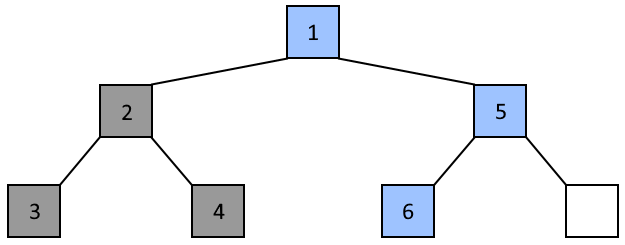
\includegraphics[width=\textwidth]{images/graph/dfs.png}}
\textit{In the above image, blue is the proper path from $1$ to $6$ while grey is explored nodes that are not involved in the proper path.}

In the above example, we start at node $1$ and want to find whether a path exists to node $6$. A DFS will begin by checking $\{1\}$, $\{1, 2\}$, $\{1, 2, 3\}$, $\{1, 2, 4\}$, $\{1, 5\}$, $\{1, 5, 6\}$, and at that point can say there is a path between $1$ and $6$. 

We can model this using a stack data structure, where we add all unvisited neighbors of a node into the stack. If at any point we encounter the end node, we know there's a valid path and can return \mintinline{cpp}{true} then. If our stack is empty, we know we've checked every node connected to our starting position without finding the end node.

\inputcpp{code/graph/dfs_stack.cpp}

A keen eye can notice that using a stack like that is very similar to recursion -- in fact the code for a DFS becomes significantly shorter when we convert it to use recursion instead:

\inputcpp{code/graph/dfs_recursive.cpp}

\subsubsection{Breadth First Search}
\index{Breadth First Search}

Breadth first search is similar to depth first search, except instead of trying to search through the first path possible (prioritizing \textit{depth}) we try to search through every neighbouring node (priorizing \textit{breadth}).

The simplest approach to implementing this is to take our stack-based implementation for DFS and use a queue instead. This means that, instead of trying the most recently added node for the next iteration as we would in a DFS, we will use the oldest node for the next iteration.

\subsubsection{Dijkstra's Algorithm}
\index{Dijkstra's Algorithm}

DFS and BFS, as can be noted, doesn't consider weighted graphs -- if we exit at the first time we encounter the target end node, DFS will give us some valid path and BFS will give us a path with the minimum number of edges. In neither case are these edges necessarily with the minimum total weight (in BFS's case, we may find a solution in one edge with weight of 100, when the minimum total weight would be two edges each with weight 1).

Dijkstra's algorithm is a solution to this. It's also implemented like DFS or BFS except we use a priority queue, where the weight of our current path is how we base the priority (we consider lower weights before higher weights). Additionally, rather than storing whether a node is visited or not, we store the current best (minimum) weight of a path we've found (defaulting to infinity, or some huge number that won't be encountered normally). Using this, when we consider the neighbors of an node, rather than checking if that node is already visited we check if our current node's best weight + the weight of our next edge, and add that to our priority queue if so.

\subsubsection{A* Algorithm}
\index{A* Algorithm}

The A* algorithm can be considered a generalization of Dijkstra's, in which we use a heuristic function to (hopefully) improve performance.

\subsubsection{Bellman-Ford Algorithm}
\index{Bellman-Ford Algorithm}

A restriction with Dijkstra's is that it can't handle negative weights properly -- there are specific cases where a negative weight can break the assumptions that Dijkstra's makes.

The Bellman-Ford algorithm can work with this, both by being able to handle negative weights (when there are no negative cycles) and being able to detect negative cycles (in which case there is no shortest path).

\subsubsection{Floyd-Warshall Algorithm}
\index{Floyd-Warshall Algorithm}

So far the algorithms we've considered have been single-source shortest path algorithms -- namely that we have a specific starting node. What if we want to determine the shortest path distance between any two arbitrary points? We would need an all-pairs shortest path algorithm instead.

Floyd-Warshall meets these requirements. It works with negative weights as well, assuming that there are no negative weight cycles.

\subsubsection{Path Reconstruction}
\index{Path Reconstruction}

For DFS, BFS, Dijkstra's, etc. we can include an auxillary array that represents some data about each node. In order for the algorithms to work, we already include an array that determines whether a node has been visited for DFS and BFS, and for Dijkstra's we include an array that determines the minimum weight of a path we've needed so far.

One of the most common ones is a \textit{parent} array, in which every node stores what node came before it in the path. This is useful for path reconstruction, where we want to determine the path taken to get to the end node.

When we set our node as visited (for DFS and BFS) or the weight required (for Dijkstra's) we also set the parent node. Then, after our algorithm is done, we check the parent of the end node, then its parent, then the parent of that node, and so on until we reach the source node. The path is this list of parents in reverse.

\subsection{Union-Find}
\index{Union-Find} \index{Disjoint-Set} \index{DSU}

Union-Find, which also goes by the name of \textit{disjoint-set}, is a data structure that groups connected nodes together into different subsets through operations called \textbf{union} (which connects two nodes together, akin to creating an edge) and \textbf{find} (which determines which subset a node belongs to). As a result, Union-Find is well suited for any problem in which you have to determine if two different elements belong to the same set -- this sees applications both by itself in many problems, and as an important part of different graph algorithms.

\subsection{Minimum Spanning Trees}
\index{Spanning Trees} \index{Minimum Spanning Trees}

Many graphs have redundant edges -- between nodes $A$ and $B$ there may be several different paths. A spanning tree of a connected graph is one in which we use a subset of edges (whether we think of it as removing redundant edges or building up only the necessary edges depends on the algorithm we use) so that every pair of nodes has exactly one unique path between them.

A minimum spanning tree is a variant of a general spanning tree, where we want to obtain the minimum total weight among all spanning trees. This is not necessarily unique either, as there easily could be multiple possible minimum spanning trees.

\subsubsection{Prim's Algorithm}
\index{Prim's Algorithm}

\subsubsection{Kruskal's Algorithm}
\index{Kruskal's Algorithm}

\subsection{Strongly Connected Components}
\index{Strongly Connected Components}

\subsubsection{Kosaraju's Algorithm}
\index{Kosaraju's Algorithm}

\subsubsection{Tarjan's Algorithm}
\index{Tarjan's Algorithm}

\subsection{Maximum Flow}
\index{Maximum Flow}

\subsection{Bipartite Graphs}
\index{Bipartite Graphs}

\subsubsection{Determining Bipartite Graphs}
\subsubsection{Maximum Bipartite Matching}
\index{Maximum Bipartite Matching}

\subsection{Eulerian Paths}
\index{Eulerian Paths} \index{Eulerian Cycles}

A Eulerian Path is a traversal of a graph in which every edge is visited exactly once. By consequence each node will also be visited one or more times.

Similarly, a Eulerian Cycle is a traversal of a graph that visits every edge exactly once with the added restriction that it's a cycle and has the same start and end node.

It is relatively easy to verify whether or not a Eulerian Path or Cycle exists. The following conditions must be satisfied:
\begin{itemize}
\item The graph must be connected
\item The degree of each node must be even
\end{itemize}

\subsubsection{BEST Algorithm}
\index{BEST Algorithm}

\subsubsection{Hierholzer's Algorithm}
\index{Hierholzer's Algorithm}

\subsection{Hamiltonian Paths}
\index{Hamiltonian Paths} \index{Hamiltonian Cycles}

A Hamiltonian Path is similar to a Eulerian Path except that it deals with nodes rather than edges -- it's a traversal in which each node is visited exactly once, and by consequence each edge is either visited once or not visited at all.

A Hamiltonian Cycle follows the same convention where we add the restriction that the end node of our traversal also has to be our source node.

Unlike Eulerian Paths and Cycles, verifying whether a Hamiltonian Path or Cycle exists or not is an NP-complete problem for the general case. There are special cases however:
\begin{itemize}
\item a complete graph with $n$ nodes has $(n-1)!/2$ different Hamiltonian Cycles.
\item By Dirac's Theorem, a simple graph with at least 3 nodes contains a Hamiltonian Cycle if every node has a degree of at least $\frac{n}{2}$ where $n$ is the number of nodes in the graph.
\item By Ore's Theorem (which generalizes Dirac's Theorem), a simple graph with at least 3 nodes contains a Hamiltonian Cycle if, for every pair of nodes in the graph, the sum of their degrees is at least $n$ where $n$ is the number of nodes in the graph.
\end{itemize}
\section{Number Theory Problems}

\subsection{Binary Exponentiation}

Consider the naive way to calculate $a^n$ (where $n$ is an integer), we simply get the product of $n$ $a$s. In terms of code, we can simply initialize a variable to $1$ and then have a for-loop that multiplies our variable by $a$ a total of $n$ times. This works fine for $0^n$ where our answer should be 0, and $a^0$ where our answer should be $1$, but doesn't work for $0^0$ which is undefined (for simplicity's sake, we'll ignore $0^0$).

\inputcpp{code/number_theory/pow_naive.cpp}

Unfortunately, this is relatively slow. In many problems or algorithms where you need to use exponentiation, calculating it in $O(n)$ is far too slow.

Binary exponentiation is the idea of calculating an arbitrary integer power as a product of different values of $a^{2^n}$. Specifically, we rely on two properties:
\begin{itemize}
\item We can represent a number as a sum of powers of 2 based on its binary representation. Consider the decimal number $10$, which has a binary representation of $1010_2$. We can tell that $10 = 2^1 + 2^3$ from its binary representation.
\item $a^{n+m} = a^n * a^m$. Rather than calculate the larger $a^{n+m}$ we can instead calculate it as the product of smaller powers that add to $n+m$.
\end{itemize}

When we combine these together, we can notice that $a^{10} = a^{2^1 + 2^3} = a^{2^1} * a^{2^3}$. What makes calculating this very fast is noticing that $a^{2^{i+1}} = (a^{2^i})^2$, so that we can quickly iterate through values of $a^{2^i}$:

\inputcpp{code/number_theory/pow_binary.cpp}

The value in this is that we have significantly reduced our runtime. Rather than calculate in $O(n)$, we calculate in $O(log_2n)$. Now, rather than $2^{2^{31}-1}$ requiring over 2 billion iterations of a for-loop in the naive method, it takes a mere 31 iterations of a while-loop in our binary exponentiation method.

\subsection{Primes}

\subsubsection{Prime Sieve}

\subsubsection{Primality Test}

\subsubsection{Prime Factoring}

\subsection{Greatest Common Divisor}

\subsubsection{Basic GCD}

\subsubsection{Extended GCD}

\subsubsection{Primal Representation}

Given a prime factorization of two numbers, the GCD is the product of factors in common. For example, the prime factorization of $60$ is $\{2,2,3,5\}$ while the prime factorization of $24$ is $\{2,2,2,3\}$. The factors in common are $\{2,2,3\}$ whose product is 12, which is the GCD of 60 and 24.

\subsubsection{Least Common Multiple}

The least common multiple between two non-zero integers can be calculated quickly: $\frac{a * b}{gcd(a, b)}$. Since $gcd(a, b)$ is a divisor of both $a$ and $b$ (and by extension $a * b$) this will always be an integer as well.

The primal representation of the LCM is similar to the primal representation of their GCD, except it's the product of factors they don't share multiplied by the product of factors in common (or GCD). For example, with $60$ and $24$ again, we have $\{2,5\}$ as unshared factors, along with $\{2,2,3\}$ as common factors, which is $2 * 2 * 2 * 3 * 5 = 120$ which is the LCM.

\subsubsection{Coprime Numbers}

Numbers are considered coprime (or relatively prime) if their GCD is 1. That is to say, they have no prime factors in common.

Prime numbers are, by necessity, coprime to other primes. This is because they would share no prime factors (for both, their sole prime factor being themselves) and as such have a GCD of 1. Following similar logic, any number is either coprime to a prime, or it's a multiple of that prime (because the only scenario that the GCD wouldn't be 1 is when the prime is a factor).

\subsection{Modular Arithmetic}

\subsubsection{Addition}

Addition can be fairly simple -- we add our numbers together and then perform the modulo operation on it. For example:

\inputcpp{code/number_theory/modulo_add.cpp}

The modulo operation is relatively expensive for a basic arithmetic operation, however. If we can guarantee that $a$ and $b$ are both less than $m$, we can avoid doing any modulo operations with:

\inputcpp{code/number_theory/modulo_add_fast.cpp}

\subsubsection{Subtraction}

Subtraction is similar to addition, but we need to guarantee that we don't go negative. We can fix this by simply adding $m$ before performing our modulo operation:

\inputcpp{code/number_theory/modulo_sub.cpp}

Likewise with addition, we can also optimize our subtraction function to not perform any modulo operation:

\inputcpp{code/number_theory/modulo_sub_fast.cpp}

\subsubsection{Multiplication}

Multiplication can (mostly) be performed similar to the non-optimized method of addition and subtraction -- by simply doing the multiplication operation and then performing the modulo operation on that. However, we may be concerned with overflows.

Specifically, consider $m = 10^9 + 7$. The largest numbers we will multiply will be when both $a$ and $b$ are equal to $10^9 + 6$. $a * b$ is somewhat above $10^{18}$ which is outside of the range of what a 32-bit integer can hold. In a language like C++ or Java, we will have to ensure that we use 64-bit integers when performing our multiplication:

\inputcpp{code/number_theory/modulo_mul.cpp}

\subsubsection{Exponentiation}

\subsubsection{Division (Prime Modulo)}

\subsubsection{Modular Inverse}

\subsubsection{Division (Any Modulo)}

\subsubsection{Discrete Log}

\subsubsection{Square Root}

\section{Combinatorics Problems}
\section{Geometry Problems}
\section{Statistics Problems}
\section{Game Theory Problems}
\index{Game Theory}

Under Construction

\subsection{Nim}
\index{Nim}

Under Construction

\subsection{Sprague-Grundy}
\index{Sprague-Grundy}

Under Construction

\subsubsection{Nimber Addition}
\index{Nimbers}

Under Construction

\subsubsection{Nimber Multiplication}

Under Construction

\subsection{Josephus Problem}
\index{Josephus Problem}

The Josephus problem is a specific task that can be formulated as:

$n$ people stand in a circle. We begin at the first person, who then excludes the person who is $k-1$ positions to the right of themselves. We then repeat the same process, starting at the person to the right of the one who was just removed. We continue until there is only one person who hasn't been excluded. Our task is to find out who that last person is.

As an example with $n = 7$ and $k = 3$, we begin with a list $\{0, 1, 2, 3, 4, 5, 6\}$. The first person removes the position 2 to the right, so we adjust our list and have $\{0, 1, 3, 4, 5, 6\}$. $3$ then removes $5$, giving us $\{0,1,3,4,6\}$. $6$ removes $1$, for $\{0,3,4,6\}$. $3$ removes $6$, $0$ removes $4$, then $0$ removes $0$. We arrive at a list of size 1, where our answer then is $3$.

The problem has some grim origins, originating from a story of a historian Flavius Josephus living in the first century, wherein himself and 40 soldiers decided to avoid capture by standing in a circle and committing suicide in a manner not unlike what was described above. The original story has some differences from the formulated problem, namely that there were two survivors rather than just one, and that Josephus claimed it luck or will of God rather that he be spared rather than intentionally calculating the safest spot, but broadly speaking it's a strong example of the Josephus problem.

\inputcpp{code/game_theory/josephus_general.cpp}

\inputcpp{code/game_theory/josephus_k2.cpp}

Under Construction

\appendix
\renewcommand{\thesubsection}{\Alph{section}.\alph{subsection}}
\renewcommand{\thesubsubsection}{\Alph{section}.\alph{subsection}.\roman{subsubsection}}

\section{Optimizations}

\subsection{Concepts}

\subsubsection{Cache Efficiency}

\subsubsection{Register Usage}

\subsubsection{Branch Prediction}

\subsubsection{Type Conversions}

\subsubsection{Data Alignment}

\subsubsection{Run-Time and Compile-Time}

\subsection{General}

\subsubsection{Avoid Additional Allocations}

\subsubsection{Bitwise Operations}

\subsubsection{Boolean Operand Order}

\subsubsection{Multidimensional Array Element Access Order}

\subsubsection{Lazy Evaluation}

\subsection{Specific Techniques}

\subsubsection{Reverse Access of Loops}

\subsubsection{Favor Simple Loop Counters}

\subsubsection{Recursion Alternatives}

\subsubsection{Distance as Distance Squared}

\subsubsection{Counting Arrays as Boolean Arrays}

\subsubsection{Multiple Divisions as Multiplication by Reciprocal}

\subsubsection{Floating Point Exceptions as NAN/INF}

\subsection{C++}

\subsubsection{Inlined and Macro Functions}

\subsubsection{Const Correctness}

\subsection{Java}

\subsection{Python}

\section{Templates}

Many competitive programmers, rather than remember the details for complicated data structures and algorithms, will save a copy of the necessary code for later reuse.

\subsection{Snippets}

Code that you intend to use for templates can differ widely from other code you write -- it's often far more generalized than what you normally write in competitive programming, which makes it like general software development in that sense. But it's also usually far more compressed with little concern about architectural decisions, much more like competitive programming than general development.

\subsection{Team Notebooks}

Currently in ICPC competitions, and many smaller-scale competitions, you are allowed a 25-page single-sided notebook containing code snippets. This section contains some recommendations for creating this.


\printindex

\end{document}